\documentclass[DIV=calc, paper=a4, fontsize=11pt]{scrartcl}	 % A4 paper and 11pt font size
%\documentclass[DIV=calc, paper=a4, fontsize=11pt, twocolumn]{scrartcl}	 % A4 paper and 11pt font size

\usepackage{multicol}
\usepackage{color}
\usepackage{lipsum}
\usepackage[italian]{babel}
\usepackage[protrusion=true,expansion=true]{microtype}
\usepackage{amsmath,amsfonts,amsthm}
\usepackage[svgnames]{xcolor}
\usepackage[hang, small,labelfont=bf,up,textfont=it,up]{caption}
\usepackage{booktabs}
\usepackage{fix-cm}
\usepackage[margin=1in]{geometry}
\usepackage[utf8]{inputenc}
\usepackage{listings}
\usepackage{url}
\usepackage{float}
\usepackage{graphicx}
\usepackage{caption}
\usepackage{subcaption}
\setlength{\columnsep}{.6cm}

\usepackage{sectsty}
\allsectionsfont{\usefont{OT1}{phv}{b}{n5}}
\usepackage{fancyhdr}
\pagestyle{fancy}
\usepackage{lastpage}

% Headers - all currently empty
\lhead{}
\chead{}
\rhead{}

% Footers
\lfoot{}
\cfoot{}
\rfoot{\footnotesize Page \thepage\ of \pageref{LastPage}} % "Page 1 of 2"

\renewcommand{\headrulewidth}{.0pt} % No header rule
\renewcommand{\footrulewidth}{.4pt} % Thin footer rule

\usepackage{lettrine} % Package to accentuate the first letter of the text
\newcommand{\initial}[1]{ % Defines the command and style for the first letter
\lettrine[lines=3,lhang=0.3,nindent=0em]{
\color{DarkGoldenrod}
{\textsf{#1}}}{}}

\usepackage{titling} % Allows custom title configuration

\newcommand{\HorRule}{\color{DarkGoldenrod} \rule{\linewidth}{1pt}} % Defines the gold horizontal rule around the title

\pretitle{\vspace{-30pt} \begin{flushleft} \HorRule \fontsize{30}{30} \usefont{OT1}{phv}{b}{n} \color{DarkRed} \selectfont} % Horizontal rule before the title

\title{Apprendimento Distribuito e un Caso di Studio: TensorFlow} % Your article title

\posttitle{\par\end{flushleft}\vskip 2em} % Whitespace under the title

\preauthor{\begin{flushleft}\large \lineskip 0.4em \usefont{OT1}{phv}{b}{sl} \color{DarkRed}} % Author font configuration

\author{Maxim Gaina e Bartolomeo Lombardi} % Your name

\postauthor{\footnotesize \usefont{OT1}{phv}{m}{sl} \color{Black} % Configuration for the institution name
\\ Lavoro di progetto per Sistemi Peer-to-Peer, Università degli Studi di Bologna % Your institution

\par\end{flushleft}\HorRule} % Horizontal rule after the title

\date{} % Add a date here if you would like one to appear underneath the title block

% Default fixed font does not support bold face
\DeclareFixedFont{\ttb}{T1}{txtt}{bx}{n}{12} % for bold
\DeclareFixedFont{\ttm}{T1}{txtt}{m}{n}{12}  % for normal

% Custom colors
\definecolor{deepblue}{rgb}{0,0,0.5}
\definecolor{deepred}{rgb}{0.6,0,0}
\definecolor{deepgreen}{rgb}{0,0.5,0}

\usepackage{listings}

% Python style for highlighting
\newcommand\pythonstyle{\lstset{
		language=Python,
		basicstyle=\ttm,
		otherkeywords={self},             % Add keywords here
		keywordstyle=\ttb\color{deepblue},
		emph={MyClass,__init__},          % Custom highlighting
		emphstyle=\ttb\color{deepred},    % Custom highlighting style
		stringstyle=\color{deepgreen},
		frame=tb,                         % Any extra options here
		showstringspaces=false            % 
}}

% Python environment
\lstnewenvironment{python}[1][]
{
	\pythonstyle
	\lstset{#1}
}
{}

% Python for external files
\newcommand\pythonexternal[2][]{{
		\pythonstyle
		\lstinputlisting[#1]{#2}}}

\begin{document}
	\maketitle
	\thispagestyle{fancy}
	% The first character should be within \initial{}
	\initial{Q}\textbf{uesto lavoro mira ad apprendere e riassumere le basi della libreria TensorFlow \cite{tf}, definita come un'interfaccia per esprimere algoritmi in ambito Machine Learning e con la possibilità di implementarli. Successivamente, l'intenzione sarà quella di esplorare le primitive offerte in ambito del calcolo distribuito, e dato un problema facilmente risolvibile tramite reti neurali, fare delle prove pratiche per ottenere una soluzione soddisfacente, usando un sistema di macchine connesse.}
	
	\begin{multicols}{2}
		\tableofcontents
		\section*{Cosa è TensorFlow}
			TensorFlow nasce dalla necessità di avere un sistema con le giuste proprietà e requisiti per \textit{allenare} e usare reti neurali in ambienti distribuiti su larga scala. La computazione di un programma scritto in TensorFlow è eseguibile su piattaforme multiple ed eterogenee con minimo o senza alcun cambiamento. Per ogni piattaforma presa in considerazione, è previsto lo sfruttamento delle risorse dei device a disposizione, con capacità di calcolo, come processori centrali e acceleratori di grafica. Le computazioni vengono espresse da flussi di dati che scorrono all'interno di un grafo, il quale, ogni nodo che lo compone, ha un proprio stato. Ulteriori obiettivi sono quelli di fornire un linguaggio \textit{flessibile}, che permetta la rapida implementazione di diversi modelli; un linguaggio il più possibile \textit{performante} nonostante la flessibilità appena citata; e forme di parallelismo con requisiti più o meno forti, anche per passare con facilità da ambienti isolati ad ambienti distribuiti.
			
			In questo paper verranno riassunte le principali caratteristiche di TensorFlow. In alcuni casi verrà citato direttamente \cite{tf} e alcuni schemi al suo interno per aiutarne la comprensione, ma senza per questo fare una semplice traduzione. Il tutto infatti verrà combinato a quanto è stato fatto nelle prove pratiche.
			
		\section{Paradigma e Concetti Base}
			\begin{figure}[H]
				\centering
				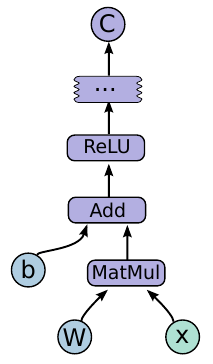
\includegraphics[scale=.9]{img/computation.png}
				\caption{Esempio di Grafo di Computazione, corrispondente alla Figura \ref{py:tfcode}}
				\label{fig:computation}
			\end{figure}
			Una computazione TensorFlow è descritta da un \textit{grafo diretto}, composto da un insieme di \textit{nodi}. Il grafo supporta computazioni che sono flussi di dati che lo attraversano. I nodi mantengono e aggiornano i propri stati persistenti tramite estensioni, che permettono quindi di creare cicli e altre strutture. Ogni nodo ha zero o più input e output ed è l'istanziazione di un'operazione. I valori che \textit{fluiscono} nel grafo sono detti \textbf{tensor}, array di dimensione $n$ nel quale ogni elemento ha un tipo determinato a tempo di costruzione del grafo. Esistono anche particolari tipi di archi, il cui unico scopo è quello di indicare le dipendenze fra nodi, cioè l'ordine di esecuzione. Vediamo ora meglio alcuni concetti.
			\begin{description}
				\item[Operazione] Avente nome e attributi, rappresenta l'astrazione di una computazione (es. \texttt{add}, \texttt{mulmatrix}, etc) su tensors in ingresso.
				\item[Kernel] Implementazione particolare di un'operazione che le permette di essere eseguito su device particolari come una \texttt{GPU CUDA}.
				\item[Sessione] I grafi dell'utente interagiscono con TensorFlow (vengono lanciati) tramite sessioni, le quali, avendo un'interfaccia, possono essere usate anche per modificare il grafo a run-time. Le sessioni hanno quindi un'operazione \textit{Run}, che prendono in input il grafo stesso e i tensori.
				\item[Variabile] I grafi vengono spesso eseguiti più volte e i tensors devono sopravvivere fra un'esecuzione e l'altra, per questo sono state create le variabili che salvano il loro valore, quando necessario. Le variabili sono anche esse tipi di nodo.
			\end{description}
			\begin{figure*}
				\pythonexternal{code/python0.py}
				\caption{Costruzione di un grafo di computazione e il suo lancio tramite sessione}
				\label{py:tfcode}
			\end{figure*}				
		
		\section{Ambienti Multi-Device e Distribuiti}
			Le componenti principali del sistema TensorFlow sono il \textit{client} e il \textit{master}. Il client usa le sessioni per comunicare con il master. Vengono usati uno o più \textit{worker process} per accedere a uno o più \textit{device} con capacità di calcolo. L'interfaccia di TensorFlow è stata implementata sia per ambiente locale che distribuito.
			\begin{description}
				\item[Locale] Client, master e worker si trovano sulla stessa macchina nel contesto di un singolo processo di sistema operativo.
				\item[Distribuito] Client, master e worker si trovano in diversi processi potenzialmente su macchine fisiche diverse.
			\end{description}
			Ogni worker è responsabile di uno o più \textit{device} (Figura \ref{py:device}), e ogni device ha il suo tipo e nome. Nello scenario del singolo device è abbastanza facile eseguire il grafo: le dipendenze fra nodi sono facilmente individuabili e l'esecuzione dei nodi viene gestita tramite una pila, secondo una politica non meglio specificata. Discorso diverso per device multipli, e quindi anche per l'ambiente distribuito.
			\begin{figure*}
				\centering
				\begin{python}
with tf.Session() as sessione:
	with tf.device("/gpu:1"):
		matrice1 = tf.constant([[3., 3.]])
		matrice2 = tf.constant([[2.],[2.]])
		prodotto = tf.matmul(matrice1, matrice2)
				\end{python}
				\caption{Vincolo di esecuzione tramite la \texttt{GPU 1} presente nel sistema}
				\label{py:device}
			\end{figure*}
			\subsection{Esecuzione su device multipli}
				Per gestire la presenza di device multipli vengono adottati nuovi accorgimenti, è infatti necessario saper decidere a quale device assegnare la computazione di un dato nodo e saper comunicare fra grafi o sottografi che si trovano in posti diversi.
				\paragraph*{Posizionamento dei nodi}\label{paragaph:partition} Una delle prime preoccupazioni di TensorFlow è quella di mappare i nodi all'insieme dei device disponibili, e viene fatto tramite un apposito \textbf{algoritmo di posizionamento}. In base ad alcune euristiche, a tempo statico viene approssimato l'input di tale algoritmo, e viene detto \textbf{modello di costo}. Per ogni nodi esso contiene la stima dei suoi tensori in input e in output espressa in byte e la stima del tempo di esecuzione. Ora che possiede l'input, l'algoritmo di posizionamento lancia un'esecuzione simulata del grafo, dove in base a euristiche \textit{greedy} è in grado di scegliere l'opportuno device.
				\paragraph{Comunicazione tra Device}\label{paragraph:communication} A questo punto ogni device all'interno del sistema ha un proprio sottografo da eseguire. Ogni arco che unisce sottografi diversi e che quindi va dal nodo $x$ a $y$, viene sostituito con un arco che va da $x$ a \textit{send} e un'altro che va da \textit{recv} a $y$. \textit{send} e \textit{recv} sono nuovi nodi introdotti che gestiscono tutti i messaggi entranti e uscenti da un sottografo (Figura \ref{fig:send-recv}).
				\begin{figure}[H]
					\centering
					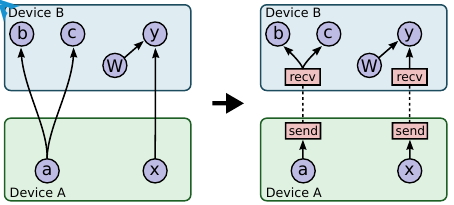
\includegraphics[scale=.75]{img/send-recv.png}
					\caption{Esempio di Grafo di Computazione, corrispondente alla Figura \ref{py:tfcode}}
					\label{fig:send-recv}
				\end{figure}
				Un po' come il corriere che si occupa di raccogliere tutte le spedizioni di una giornata, le porta in un'altro stato e le distribuisce ai relativi destinatari. Questo approccio permette di trasmettere dati una sola volta; permette che la memoria che spetta a un tensor sia allocata una sola volta anzi che più, e che nonostante il posizionamento dei nodi, l'utente possa esplicitamente assegnare l'esecuzione di un nodo a un determinato device (Figura \ref{py:device}).
			\subsection{Esecuzione Distribuita}
				L'approccio adottato per l'esecuzione distribuita di un grafo è quasi identico a quello preservato per i device. Qui la comunicazione tra grafi avviene tramite protocollo \texttt{TCP} o \texttt{RDMA}. Un'altra differenza è che negli ambienti distribuiti urge riflettere a una gestione degli errori di comunicazione. Gli errori possono avvenire tra i nodi \textit{send} e \textit{recv}, quindi è necessario verificare la salute degli scambi fra questi. Quando un fallimento viene rilevato l'esecuzione dell'intero grafo viene riavviata, ma questo non implica la perdita dei dati: si ricordi che i nodi variabile immagazzinano i tensors. Periodicamente vengono creati dei check-point dato che i nodi variabili sono collegati a speciali \textit{save node}, quindi è possibile ricoverare stati di esecuzione precedenti.
		\section{Calcolo Distribuito del Gradiente}
			Essendo TensorFlow dedicato all'apprendimento automatico, il basilare modello di programmazione comprende alcuni strumenti specializzati. In ambito di Machine Learning molti algoritmi di apprendimento calcolano il gradiente di una funziona costo, e così TensorFlow supporta il suo calcolo automatico. A livello di grafo, si supponga che un tensor $C$ dipenda (tramite un complesso sottografo di operazioni) da un insieme di tensori $\{X_k\}$, allora è disponibile una funziona che ritorna i tensors $\{dC/dX_k\}$. Dato che trattiamo il Machine Learning e l'esecuzione di un grafo che può essere distribuito, verrà vista in maniera più approfondita tale estensione.
			
			Supponiamo che la situazione sia quella di dover computare il gradiente di un tensor $C$ rispetto al gradiente di un tensore $I$. Ecco quanto accade:
			\begin{enumerate}
				\item viene trovato il cammino fra $I$ e $C$ all'interno del grafo;
				\item si va a ritroso da $C$ a $I$ e per ogni nodo operazione viene aggiunto un nuovo nodo al grafo di computazione, che computa la funzione gradiente per la relativa operazione sul cammino di ritorno;
				\begin{enumerate}
					\item la funzione gradiente può prendere in input non solo gradienti parziali computati a ritroso ma anche, opzionalmente, gli input e gli output delle relative operazioni.
				\end{enumerate}
				\item ma un'operazione $O$ può avere un insieme $E$ di archi uscenti (risultati di output) e $C$ può dipendere da un sottoinsieme di $E$: allora la funzione gradiente di $O$ prenderà in input $dC/de_k = 0$ per ogni arco $e_k$ da quale $C$ risulta \textit{indipendente};
			\end{enumerate}
			Il procedimento appena descritto si può intuitivamente osservare nella Figura \ref{fig:gradients}, che riguarda la seguente istruzione:
			\begin{center}
				\texttt{[db,dW,dx] = tf.gradients(C, [b,W,x])}
			\end{center}
			\begin{figure}[H]
				\centering
				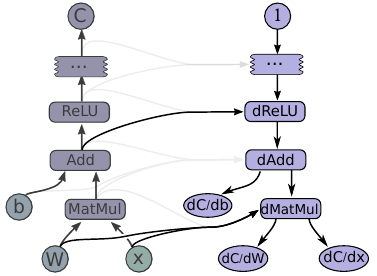
\includegraphics[scale=.9]{img/gradients.png}
				\caption{Esempio di computazione di funzione gradiente}
				\label{fig:gradients}
			\end{figure}
		
				\subsection{Controllo del flusso in ambiente distribuito}
				Il calcolo del gradiente viene considerato come estensione di TensorFlow. Altre estensioni sono: esecuzione parziale del grafo, dove l'utente sceglie quali nodi eseguire; vincoli di collocamento di un nodo (i quali sono già stati accennati), tramite i quali l'utente costringe un nodo a essere eseguito su un particolare device; controllo del flusso di esecuzione, che è un insieme di primitive che permettono di manipolare l'esecuzione del grafo (costrutti \texttt{if}, cicli \texttt{while}, \texttt{Switch}, \texttt{Merge}, ecc...); nodi \textit{feed}, che fungono da fonte di tensors per altri nodi; \texttt{queue} che permettono l'esecuzione asincrona del grafo; \texttt{containers} per gestire gli stati all'interno del grafo, e altre. Per approfondimenti si può vedere \cite{tf}.
				
				Verrà spesa in questa sede più attenzione al controllo del flusso in quanto \textbf{cruciale in ambiente distribuito}. Viene usato un importante meccanismo di coordinazione distribuita. Questo nasce dalla necessità di gestire l'esecuzione \textit{loop} che riguardano nodi assegnati a differenti device o macchine, il loro stato va infatti in qualche modo mantenuto. La soluzione che propone TensorFlow è quella della \textit{riscrittura del grafo}: durante il partizionamento dei nodi (Sottosezione \ref{paragaph:partition}), un nodo di controllo viene aggiunto per ogni sottografo. I nodi di controllo implementano una \textit{macchina a stati} che orchestra lo start e la fine di ogni iterazione, oltre alla terminazione del loop stesso. Per ogni iterazione, il device che possiede il predicato della terminazione del loop spedisce un messaggio di controllo verso tutti gli altri device coinvolti. Questi accorgimenti sono necessari anche per computare il gradiente precedentemente visto, in quanto è necessario sapere, per esempio, quale ramo di un \textit{if-then-else}	è stato imboccato per arrivare a $C$; oppure quante iterazioni sono state fatte da un particolare loop o quali erano i valori intermedi.
		
		\section{Forme di Parallelismo}
		
		\section{Ottimizzazioni e Strumenti}
		Per completezza verranno citate, ma non approfondite, alcune caratteristiche di TensorFlow che non risultano di primaria importanza in questo lavoro di progetto.
		
		Il sistema presenta alcuni accorgimenti per incrementare le performance e la gestione delle risorse. TensorFlow è in grado di invididuare pezzi di grafo ridondanti che fanno \textit{la stessa cosa} ed eliminarli, preservando la semantica del programma; può effettuare un controllo diretto dell'utilizzo della memoria e l'attivazione dei nodi di tipo \textit{recv} (Sottosezione \ref{paragraph:communication}), secondo politiche \texttt{as-soon-as-possible} oppure \texttt{as-late-as-possible}; implementa kernel non bloccanti e introduce librerie ottimizzate per lo svilippo di kernel.
		
		Viene offerto un insieme di strumenti chiamato \texttt{TensorFlowBoard}. Esso permette agli utenti di esplorare graficamente la struttura del grafo di computazione e l'analisi del suo comportamento; aiuta la visualizzazione degli stati interni e traccia le performance.
		
		\section{Apprendimento distribuito: test empirici}
		
		\section{Appunti Bart}		
		Dopo svariate prove con la libreria, ci siamo posti come obiettivo, di parallelizzare la fase di training in modo asincrono, mettendo a disposizione le risorse di tre macchine, impostate come worker, e una per gestire il tutto, settata come parameter server. Facendo uso di una rete sigmoidea con una bassa frequenza di apprendimento, abbiamo misurato le diverse performance su MNIST. L'obiettivo non è stato quello di ottenere un'alta accuratezza dopo la fase di training, ma apprendere le funzionalità della libreria.
		Il primo test valutativo, è stato quello di addestrare la rete per 20 epoche, usando un solo worker, con un risultato del 29\% di accuratezza. L'accuratezza è incrementata quando abbiamo aggiunto alla rete altre due macchine settate come worker.
			\subsection{Addestramento distribuito}
				Ci sono differenti modi per addestrare una rete in ambienti distribuiti. L'approccio più semplice è quello di condividere tutto il modello dei parametri attraverso tutti i worker mentre i dati vengono parallelizzati e il gradiente viene aggiornato. In un modello sincrono, alcuni gruppi vengono processati nello stesso lasso di tempo. Una volta che tutti i worker all'intero della rete hanno processato e terminato la fase di training, viene effettuata la media del tempo impiegato e vengono applicati gli aggiornamenti dei parametri, una sola volta. In un modello asincrono, ogni worker aggiornerà il modello dei parametri una volta che ha terminato la propria fase, senza aspettare gli altri. Durante la nostra fase di prova abbiamo usato un modello sincrono, poiché la regolazione dei parametri risultava molto complessa.
				\begin{figure}[H]
				\centering
				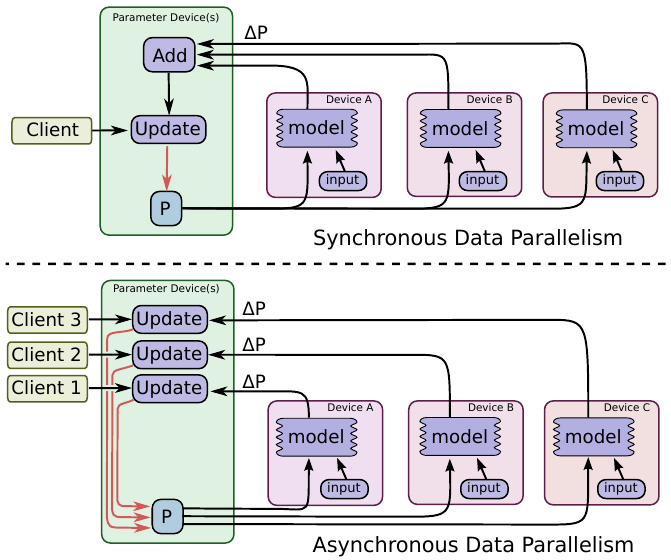
\includegraphics[scale=.55]{img/sync-async.png}
				\caption{Fase di training parallelizzata: sincrono e asincrono.}
				\label{fig:sync-async}
				\end{figure}
			\subsection{Implementazione}
				E' importante che ogni macchina del cluster conosca se stessa e le altre che ne fanno parte. Lo script implementato non parte fino a quanto tutte le macchine all'interno del nostro cluster sono online. Le specifiche del cluster sono le stesse per ogni macchina e solitamente sono costituite da parameter server e worker. Mentre il parameter server mantiene solamente i parametri condivisi, i worker effettuano i calcoli per il grafo.
				\begin{figure*}
				\pythonexternal{code/cluster.py}
				\caption{Specifiche per il cluster.}
				\label{py:clustercode}
				\end{figure*}
				ps e i worker sono chiamati \textbf{jobs} i quali, fondamentalmente, sono contenitori per uno o più \textbf{task}. Il task è il processo che il worker elaborerà durante la fase di training, volendo, è possibile aggiungere più task sulla stessa macchina. Questo potrebbe aver senso, in una macchina con più GPU, in questo modo tutti i task avranno un grafo completo del modello, ma se volessimo parallellizare il modello anzichè i dati, dovremmo cambiare il comportamento di ogni task, più nello specifico le operazioni che deve eseguire ogni task.
				Nella parte di codice \ref{py:inputflags}, andiamo a inizializzare le macchine per l'esecuzione. 
				\begin{figure*}
				\pythonexternal{code/inputflags.py}
				\caption{Specifiche per il cluster.}
				\label{py:inputflags}
				\end{figure*}

		\begin{thebibliography}{9}
			\bibitem{tf}
			Google Research,
			\emph{TensorFlow: Large-Scale Machine Learning on Heterogeneous Distributed Systems},
			Preliminary White Paper,
			2015.
		\end{thebibliography}
	\end{multicols}

\end{document}